\ylDisplay{Läätsede süsteem} % Ülesande nimi
{EFO žürii} % Autor
{piirkonnavoor} % Voor
{2020} % Aasta
{P 10} % Ülesande nr.
{3} % Raskustase
{
% Teema: Valgusõpetus
\ifStatement
Jüri tahtis ekraanile tekitada küünlaleegi suurendatud kujutist. Ta paigutas kumerläätse küünlaleegist kahekordse fookuskauguse kaugusele. Lähemale küünlale ta läätse panna ei saanud. Tekkinud kujutis ei olnud suurendatud. Jüri leidis kapist nõgusläätse ja asetanud selle kumerläätse ja ekraani vahele, saigi ekraanile küünlaleegi suurendatud kujutise. Joonistage valguskiirte käik Jüri katses ja vastake järgmisele küsimusele. Kuidas sõltub sellise skeemi korral kujutise suurus nõgusläätse fookuskaugusest?
\fi
\ifHint
Nõguslääts tuleks paigutada kumerläätse taha enne kumerläätse poolt tekitatud kujutist, nii et kumerläätse kujutis jääks nõgusläätse ja selle tagumise fookuse vahele.
\fi
\ifSolution
Konstrueerime kujutise kumerläätsega. Konstrueerime kujutisenõgusläätsega: optilised kõrvalteljed, fokaaltasand, kiired. Leiame nõgusläätsele sobiva asukoha. Joonestame läätsede süsteemi abil tekkinud kujutise. Nõguslääts tuleks paigutada kumerläätse taha enne kumerläätse poolt tekitatud kujutist, nii et kumerläätse kujutis jääks nõgusläätse ja selle tagumise fookuse vahele. Kui siin kasutatud nõgusläätse fookuskaugus on väiksem, on tekkinud kujutis suurem.
\begin{center}
	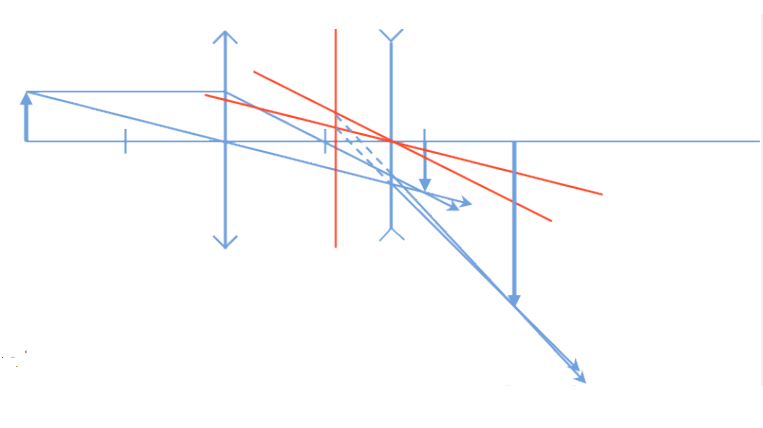
\includegraphics[width=0.5\linewidth]{2020-v2p-10-lah.PNG}
\end{center}
\fi
}
